\section{Konzeption eines an die spezifischen Probleme angepassten Workflows}

\subsection{Vorraussetzung / Abgrenzung}

Content-Management-Systeme bzw. Redaktionssystem können einen Teil der Aufgabe abbilden, sind aber i.d.R. ungeeignet (z.B. kein Workflow), keine Context-Informationen hinterlegbar.

\subsection{Workflow}

Beschreibung des optimalen Workflows und die Rolle der Beteiligten

Innerhalb der Anwendung wird das Projekt angelegt und die dafür benötigten Textbausteine definiert. Hierbei können detaillierte Angaben zu deren Eigenschaften gemacht werden, z.B. über den Verwendungszweck oder die maximal Länge. Die einzelnen Textbausteine werden bei diesem Vorgang entsprechend dem Aufbau des Endproduktes in eine Reihenfolge gebracht und hierarchisch angeordnet. So wird eine leichte Orientierung und Zuordnung der Text zum Endprodukt möglich. 

Nachdem die benötigten Textbausteine definiert wurden, werden diese durch Texter befüllt. Für Texter stellt die Anwendung Hilfsfunktionen zur Verfügung. Dazu zählen Informationen wie Zeichenlänge und Wortanzahl und Rechtschreibkorrektur mit Wörterbuch.

Sobald die Texte hinterlegt wurden durchlaufen sie die Qualitätskontrolle durch andere Mitarbeiter des Projektes und anschließend den Freigabeprozess beim Kunden. Wurden die Texte freigegeben, können die zusammengestellten Texte in das Endprodukt übernommen werden. 

Alle Vorgänge werden innerhalb der Anwendung protokolliert und sind so für jeden Beteiligten leicht nachvollziehbar. Aufgaben können automatisch aufgrund von Änderungen erzeugt werden, oder von Mitarbeiter angelegt werden. So wird sichergestellt, dass alle Projektmitarbeiter jederzeit über ihre Aufgaben bezüglich der Texte informiert sind, bei Änderungen die verantwortlichen Mitarbeiter informiert werden. Dadurch wird es möglich auch bei Korrekturen in letzter Minute diese Änderungen gezielt und transparent zu übernehmen.

\subsection{Beschreibung der notwendigen Funktionalität}

Unterteilung in Muss- und Kann-Kriterien

\subsection{Nachteile/Risiken des Konzepts}

\subsection{Personas}

Vorstellung (basierend auf Interviews mit realen Personen), Analyse des Konzepts in Bezug auf Personas

\subsubsection{Texter}

Copywriter sind die eigentlichen Texter, die lediglich Text erstellen, für die kein Fachwissen nötig ist, oder dieses schon vorliegt. Copywriter können Spezialwissen bezüglich SEO haben. Redakteure sind für die Gesamtheit der Texte verantwortlich und stellen sicher, dass globale Vorgaben erfüllt werden. Journalisten erstellen Texte, die auf Recherchen basieren. Diese Texte unterliegen der Sorgfaltspflicht, Quellen müssen nicht genannt werden. 

\section{Entwurf einer Anwendung}

Diese vier Leitlinien repräsentieren die Grundgedanken bei der Entwicklung von der Anwendung:

\begin{itemize}
\item{Das wichtigste zuerst: Die aktuelle Aufgabe soll immer im Fokus der Darstellung liegen.}
\item{Schnell zum Ziel: Alle Aufgaben müssen leicht und umkompliziert durchführbar sein.}
\item{Nicht nerven: Ständige Benachrichtigungen lenken ab und müssen deswegen so gestaltet sein, dass diese sich nach den Präferenzen des Nutzers richten.}
\item{Hilfe nur einen Klick entfernt: Das Hilfesystem muss kontextsensitiv verfügbar sein und ist eine Kernfunktion der Anwendung}
\end{itemize}

\subsection{Überblick}

Diese Abbildung liefert einen Überblick über den Aufbau des Systems:

\begin{figure}[htb]
\begin{center}
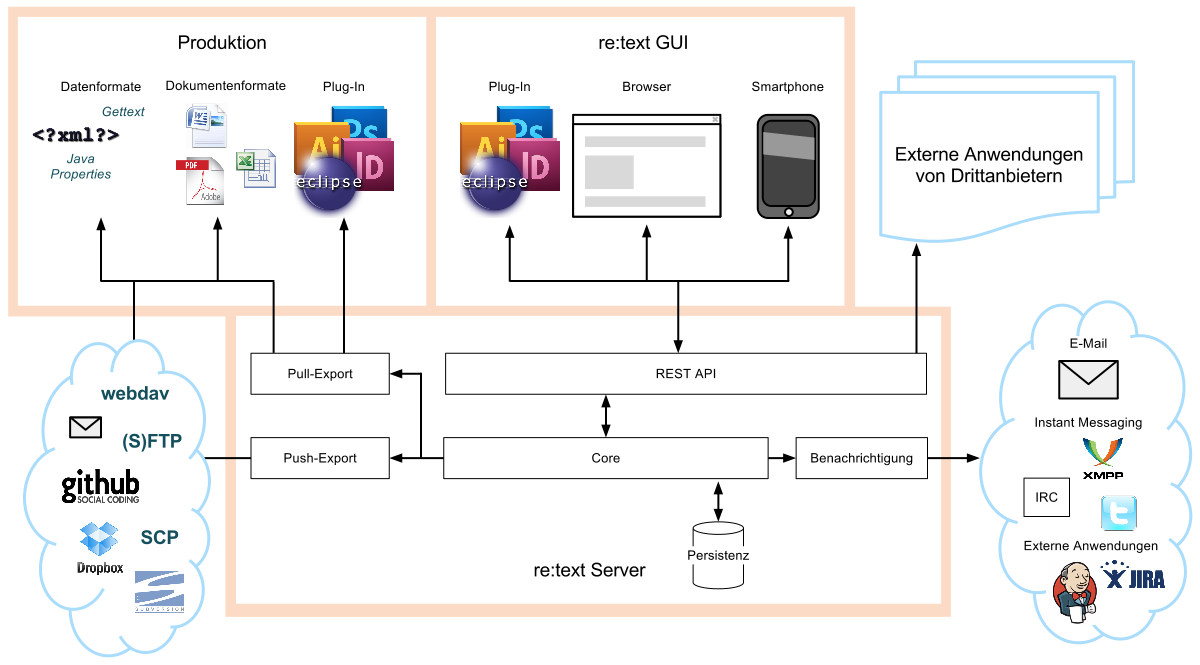
\includegraphics[width=\textwidth]{media/System.pdf}
\caption{Aufbau des Systems}
\label{chart:1}
\end{center}
\end{figure}

Die Zentrale Komponente der Anwendung bildet der Server. Für die Benutzer erfolgt der Zugriff mit Hilfe einer GUI, die mit der REST-API des Servers kommuniziert. In der ersten Version wird eine browserbasierte GUI auf Basis von HTML5 und JavaScript existieren, die auch schon auf Smartphones verwendet werden kann. Später kommen dann spezielle Plugins für Adobe-Produkte und weitere wichtige Produktionsumgebungen hinzu. Auch native GUIs für Smartphones verwenden die gleiche API. Die Schnittstellen können auch von Drittanbietern dazu verwendet werden, eigenen Clients für das System zu entwickeln. In die Endprodukte gelangen die Texten über den Export, exportiert wird dabei in viele Formate, neben Datenformaten wie z.B. XML werden auch Dokumentenformate wie z.B. Word exportiert. Der Export kann durch den Anwender erzeugt werden (\emph{Pull-Export}), aber auch automatisch, z.B. nach festgelegten Zeitplänen oder Ereignissen erfolgen. Dieser \emph{Push-Export} erfolgt auf je nach Projekt festlegbaren Orte, wie z.B. FTP-Server oder Versionsverwaltungssysteme. Die Benachrichtigungen über Aufgaben und Änderungen an Texten kann via E-Mail, aber auch mittels Instant-Messaging-Systeme oder durch den Aufruf fremde API-Endpunkte erfolgen – dies ist ebenfalls innerhalb eines Projektes und pro Nutzer individuell konfigurierbar.

\subsection{Schnittstellen}

Anforderungen, Umfang, Ausprägung für Import-, Export- und Benachrichtigungsschnittstellen

Anbindung via CMIS http://en.wikipedia.org/wiki/Content\_Management\_Interoperability\_Services

Export eines Text-Booklets für die Rechtschreibkontrolle. Identifier mit ausgeben, um Texte dann schnell finden zu können. Hier könnte man auch einen QR-Code drucken, dann kann man mit einer mobilen App den Text direkt ändern.

\subsection{Grundüberlegung zu einer GUI}

Anforderungen, Grundsätze, Usability, Aufbau, Wireframes

Bei Kontroll-Aufgaben (Lektorat, QS) unterbrechungsfreies Arbeiten ermöglichen (Infinite-Scroll).